\let\negmedspace\undefined
\let\negthickspace\undefined
\documentclass[journal]{IEEEtran}
\usepackage[a5paper, margin=10mm, onecolumn]{geometry}
%\usepackage{lmodern} % Ensure lmodern is loaded for pdflatex
\usepackage{tfrupee} % Include tfrupee package

\setlength{\headheight}{1cm} % Set the height of the header box
\setlength{\headsep}{0mm}     % Set the distance between the header box and the top of the text

\usepackage{gvv-book}
\usepackage{gvv}
\usepackage{cite}
\usepackage{amsmath,amssymb,amsfonts,amsthm}
\usepackage{algorithmic}
\usepackage{graphicx}
\usepackage{textcomp}
\usepackage{xcolor}
\usepackage{txfonts}
\usepackage{listings}
\usepackage{enumitem}
\usepackage{mathtools}
\usepackage{gensymb}
\usepackage{comment}
\usepackage[breaklinks=true]{hyperref}
\usepackage{tkz-euclide} 
\usepackage{listings}
% \usepackage{gvv}                                        
\def\inputGnumericTable{}                                 
\usepackage[latin1]{inputenc}                                
\usepackage{color}                                            
\usepackage{array}                                            
\usepackage{longtable}                                       
\usepackage{calc}                                             
\usepackage{multirow}                                         
\usepackage{hhline}                                           
\usepackage{ifthen}                                           
\usepackage{lscape}
\usepackage{circuitikz}
\tikzstyle{block} = [rectangle, draw, fill=blue!20, 
    text width=4em, text centered, rounded corners, minimum height=3em]
\tikzstyle{sum} = [draw, fill=blue!10, circle, minimum size=1cm, node distance=1.5cm]
\tikzstyle{input} = [coordinate]
\tikzstyle{output} = [coordinate]


\begin{document}

\bibliographystyle{IEEEtran}
\vspace{3cm}

\title{1.5.14}
\author{EE25BTECH11026-Harsha}
 \maketitle
% \newpage
% \bigskip
{\let\newpage\relax\maketitle}

\renewcommand{\thefigure}{\theenumi}
\renewcommand{\thetable}{\theenumi}
\setlength{\intextsep}{10pt} % Space between text and floats


\numberwithin{equation}{enumi}
\numberwithin{figure}{enumi}
\renewcommand{\thetable}{\theenumi}

\textbf{Question}:\\
Points P and Q trisect the line segment joining the points A $\brak{-2, 0}$ and B$\brak{0,8}$ such that P is nearer to A. Find the coordinates of points P and Q.\\ 
\solution \\
Let us solve the given equation theoretically and then verify the solution computationally \\
According to the question, \\
Let the vectors $\vec{P}$ and $\vec{Q}$ be 
\begin{align}
    \vec{P}=\begin{myvec}{x_1\\y_1}\end{myvec} \;, \vec{Q}=\begin{myvec}{x_2\\y_2} \end{myvec}
\end{align}
Given the points,
\begin{align}
    \vec{A}=\begin{myvec}{-2\\0}\end{myvec}
    \vec{B}=\begin{myvec}{0\\8}\end{myvec}
\end{align}
we can use the internal division formula to find the vectors $\vec{P}$ and $\vec{Q}$.\\
\textbf{Internal division formula for a vector $\vec{R}$ which divides the line formed by vectors $\vec{A}$ and $\vec{B}$ in the ratio m:n is given by}
\begin{align}
    \vec{R}=\frac{m\vec{B}+n\vec{A}}{m+n}
\end{align}
To find vector $\vec{P}$, as it is near the point A, it divides the line formed by line A and B in ratio 1:2. Therefore,\\
\begin{align}
    \vec{P}=\frac{2\times\begin{myvec}{-2 \\ 0}\end{myvec}+1\times\begin{myvec}{0\\8}\end{myvec}}{1+2}
\end{align}
\begin{align}
    \vec{P}=\begin{myvec}{\frac{-4}{3}\\\frac{8}{3}}\end{myvec}
\end{align}

To find vector $\vec{Q}$, as it is near the point B, it divides the line formed by line A and B in ratio 2:1.Therefore,\\
\newpage
\vspace*{0.25cm}


\begin{align}
    \vec{Q}=\frac{1\times\begin{myvec}{-2 \\ 0}\end{myvec}+2\times\begin{myvec}{0\\8}\end{myvec}}{2+1}
\end{align}
\begin{align}
    \vec{Q}=\begin{myvec}{\frac{-2}{3}\\\frac{16}{3}}\end{myvec}
\end{align}
\\
From the figure it is clearly verified that the theoretical solution matches with the computational solution.\\
\begin{figure}[h!]
    \centering
    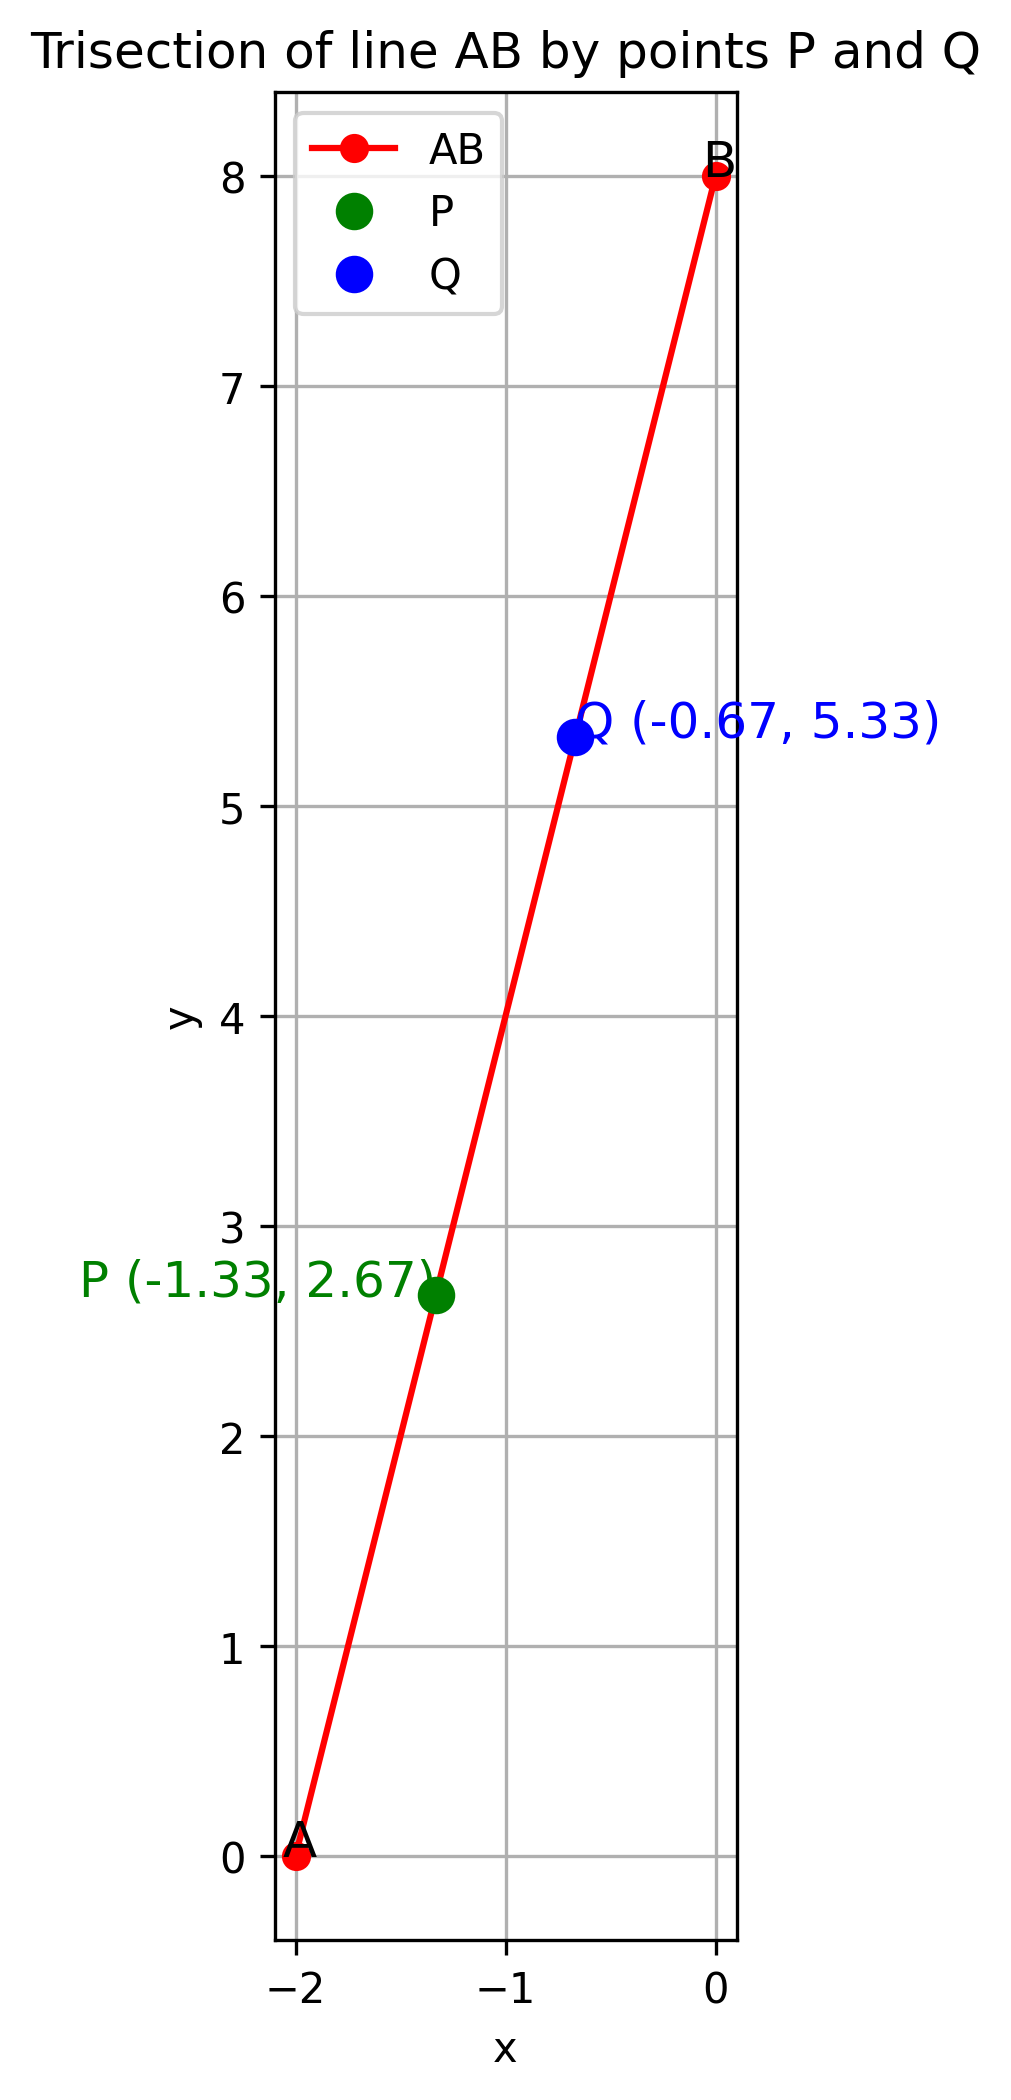
\includegraphics[height=0.5\textheight, keepaspectratio]{figs/Figure_1.png}
    \label{figure_1}
\end{figure}
 


\end{document}


